\chapter{Software Testing}

\section{Test-Prozess}

Innerhalb des Test-Prozess arbeiten mehrere Personen mit unterschiedliche Rollen:

\begin{description}
	\item[Testmanager (Führung)] Ansprechpartner für PL und Managemenet in kritischen Phasen. Plant Ressourcen, sucht verschiedene Lösungen und bewertet sie. Kann Leute führen. Entwickelt Teststrategien.
	\item[Testarchitekt, Testengineer (Ingenieur)] Plant und entwickelt die Testinfrastruktur. Entwickelt und verbessert Testmethoden und Testwerkzeuge. Entwickelt Teststrategien.
	\item[Testanalyst (Ingenieur)] Leitet aus Anforderungen Testszenarien ab. Entwickelt komplexe Testabläufe. Bestimmt Testdaten.
	\item[Testdatenverantwortlicher (Informatiker)] Pflegt, verwaltet, bewirtschaften und erweitert die Testdaten mittels Tools. Schnittstelle zwischen Testanalysten, Fach und IT. 
	\item[Tester (Fachperson)] Führt zuverlässig und exakt Tests aus. Dokumentiert präzis und wertfrei/neutral die Ergebnisse sowie die Abweichungen. Kann reproduzieren.
\end{description}

Wie die Abbildung \ref{fig:test-prozess} zeigt, ist der Test-Prozess (nach Noser) in vier Schritte eingeteilt.

\begin{figure}[h!]
\centering
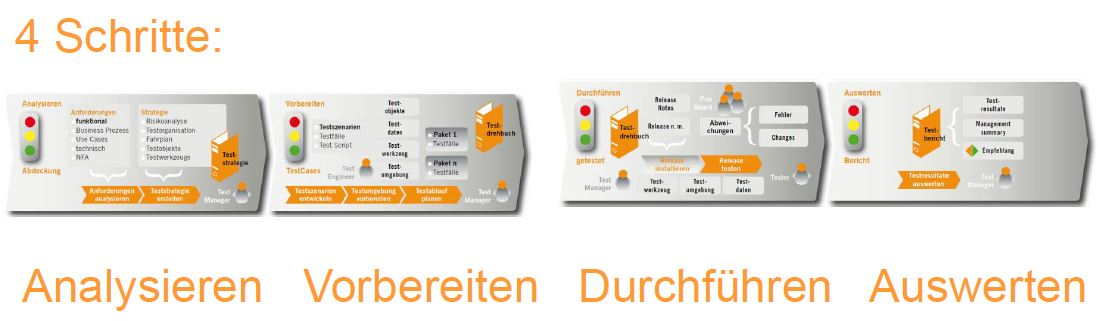
\includegraphics[width=0.7\linewidth]{fig/test-prozess}
\caption{Test-Prozess}
\label{fig:test-prozess}
\end{figure}

\subsection{Schritt 1: Analysieren}

\begin{quote}
	Wie können die Entwickler entwickeln, wenn die Tester nicht wissen, was zu testen ist?
\end{quote}


\begin{figure}[h!]
\centering
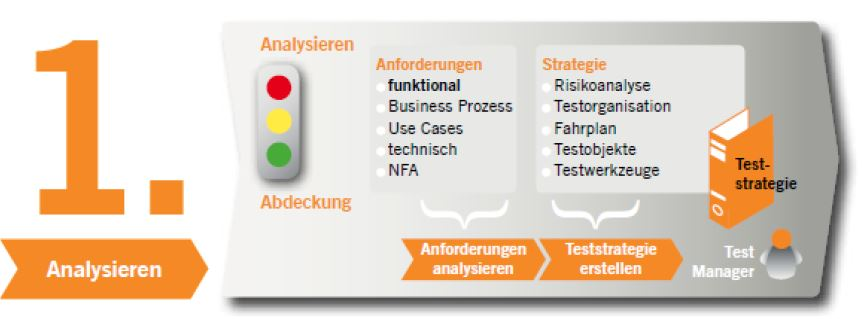
\includegraphics[width=0.7\linewidth]{fig/test-prozess-schritt-1}
\caption{Test-Prozess Schritt 1}
\label{fig:test-prozess-schritt-1}
\end{figure}

\textbf{Testen braucht eine Strategie}. Die Teststrategie bestimmt ob, was und wie tief getestet werden soll. Wo liegt der Fokus? Preis, Durchlaufzeit, Security, Usability, Performance, etc.? Vorgängig soll man sich darüber Gedanken machen und diese verbindlich festhalten. In der Teststrategie wird das Test-Vorgehen, verantwortliche Personen sowie den Prozess und die Hilfsmittel definiert. 

Warum ein Risiko basiertes Testen: Oft bleibt in kritischen Phasen nicht genug Zeit um \emph{alles} zu testen. Daher pro Iteration entscheiden, was in welchem Umgang getestet wird - kategorisieren und priorisieren. Nachfolgend werden drei Kritieren mit einem Wert von 1-3 bewertet. Das Produkt daraus gibt den Risiko Prioritäts Index (RPI):

\begin{itemize}
	\item Business Relevanz: Auswirkung bei Fehler, wie schlimm ist ein Fehler (3 = am schlimmsten)
	\item Auffindbarkeit: Wie schnell wird ein Fehler entdeckt? (1 = leicht erkennbar)
	\item Komplexität: Wie komplex ist die Anforderung und die Lösung dazu? (3 = sehr komplex)
\end{itemize}

\begin{figure}[h!]
\centering
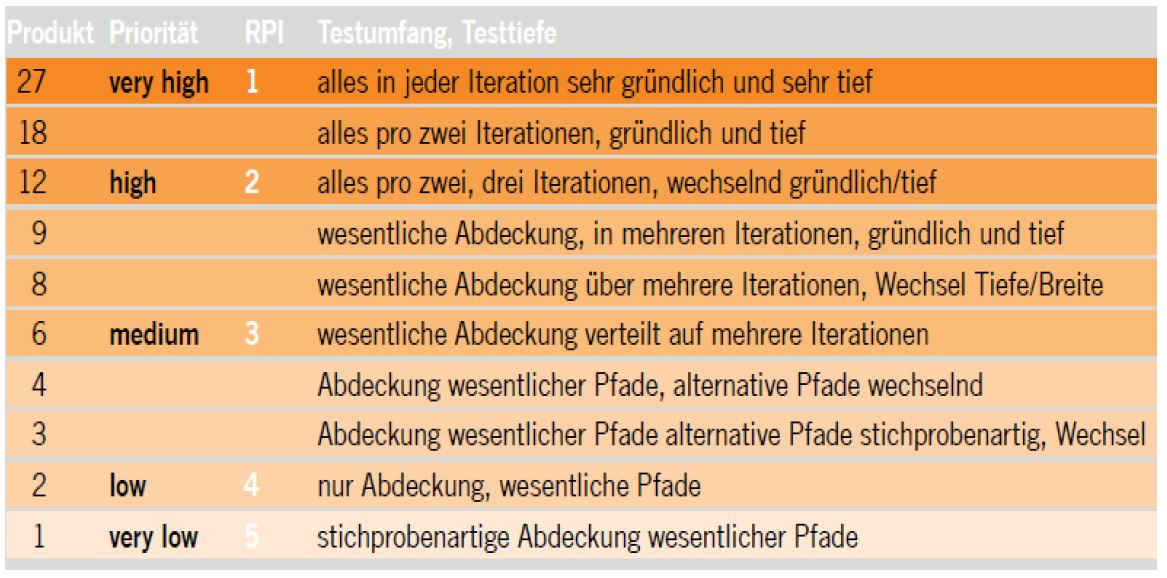
\includegraphics[width=0.8\linewidth]{fig/rpi-skala}
\caption{RPI-Skala}
\label{fig:rpi-skala}
\end{figure}

Der RPI definiert die Testtiefe, den Testumfang und die Anzahl der Wiederholungen. Somit ist der RPI das wichtigste Steuerungs- und Führungsinstrument.

Nebst dem Risiko basierten Testen gibt es noch andere Teststrategien:

\begin{itemize}
	\item ISO 29119: Was umfasst Qualität. Umfassende und ganzheitliche Betrachtung. Nach Vorlagen - Rad nicht neu erfinden.
	\item V-Modell: Tests auf jeder Stufe. Fehler so früh wie möglich entdecken.
	\item RPI: Risikiobasiertes Testen. So wenig wie möglich, aber das wo nötig.
	\item Kosten-Nutzen: Risikoabwägung. Welches Risiko wollen wir tragen, was darf es kosten?
\end{itemize}

Nebst dem Vorgehen spielen auch die \textbf{Tools} eine wichtige Rolle. Welche Tools werden für die Verwaltung von Anforderungen, Tests, Testabläufe und Testplanung verwendet. Mit was macht man Bug-Tracking, manuelles Testen, automatisiertes Testen, Lasttest, Datenmanipulation, Datengenerierung? Für alle Tools sollte man sicher immer Gedanken machen. Was ist das Ziel, wer kann das Tool bedienen, wie sieht die Lebensdauer aus, Kosten, wartbar, etc.

\subsection{Schritt 2: Vorbereiten}

\begin{quote}
	Tester und Q-Menschen sind nie bereit, sie können die Testvorbereitung sowie die Testinfrastruktur problemlos vergolden.
\end{quote}

\begin{figure}[h!]
\centering
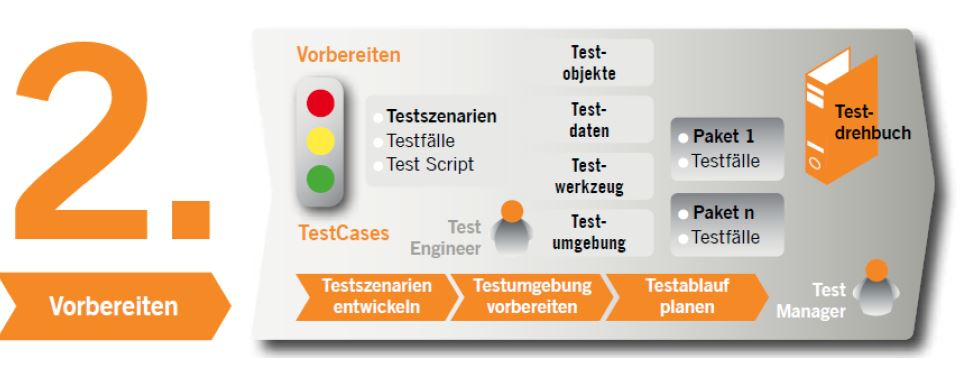
\includegraphics[width=0.7\linewidth]{fig/test-prozess-schritt-2}
\caption{Test-Prozess Schritt 2}
\label{fig:test-prozess-schritt-2}
\end{figure}

Die Vorbereitungsphase legt die Basis für den Erfolg:

\begin{itemize}
	\item Test-Infrastruktur
	\item Test-Team (keine Diletanten!)
	\item Test-Daten
	\item Test-Automaten, Test-Automatisierung
	\item Eskalationswege
	\item NFA-Test
	\item Test-Stufen
	\item Test-Szenarien, Test Cases, Test-Fälle
\end{itemize}

\begin{figure}[h!]
\centering
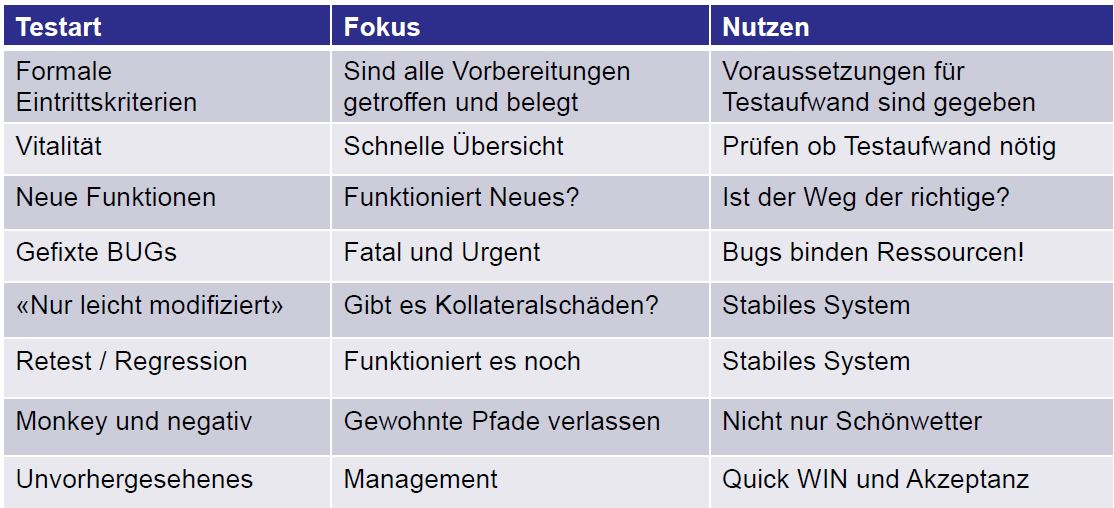
\includegraphics[width=0.7\linewidth]{fig/testarten-zur-planung}
\caption{Testarten zur Planung}
\label{fig:testarten-zur-planung}
\end{figure}

Mittels Blackbox-Test wird das Ein- und Ausgabeverhalten überprüft. Dabei kann die Anzahl der Testfälle explodieren. Mittels Whitebox-Test werden die interne Logik des Systems oder Objekts angeschaut. 

Die Codeabdeckung ist eine Metrik, welche die die durch Tests erreichte Codeabdeckung beschreibt. Damit können die benötigten Testfälle ermittelt werden. Es gibt unterschiedliche Abdeckungen:
\begin{description}
	\item[Anweisungsüberdeckung] Jede Anweisung wird mind. 1 mal aufgerufen.
	\item[Zweig-, Entscheidungsabdeckung] Jeder Eintritt- und Austrittspunkt wird mind. einmal durchlaufen.
	\item[Pfadabeckung] Pfade im Code.
\end{description}

Wir können nicht alles testen, da es unzählige Pfade gibt. Wir brauchen eine Strategie, welche risikobasiert ist um die Frage zu beantworten, wie viel und wie tief getestet werden soll.

\subsection{Schritt 3: Durchführen}

\begin{quote}
	Die Praxis zeigt immer wieder, dass von Hand gepflegte Systeme in kritischen Momenten nicht mehr gepflegt werden, denn Testen geht immer vor. Doch genau dann sind die Kennzahlen als Entscheidungsbasis besonders wichtig.
\end{quote}

\begin{figure}[h!]
\centering
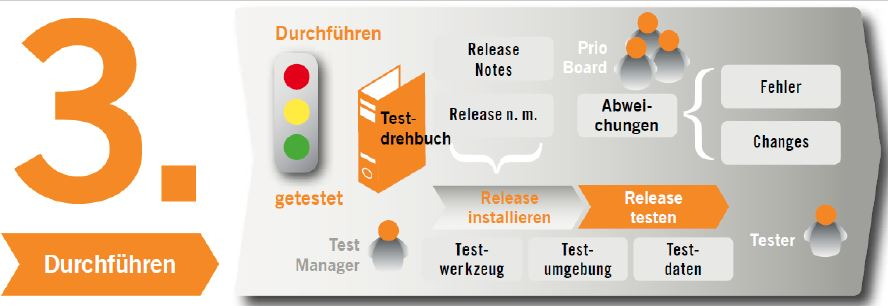
\includegraphics[width=0.7\linewidth]{fig/test-prozess-schritt-3}
\caption{Test-Prozess Schritt 3}
\label{fig:test-prozess-schritt-3}
\end{figure}

Auf Abbildung \ref{fig:wichtigkeit-des-testen} sieht man, dass sowohl der linke untere Quadrant und der rechte obere Quadrant dasselbe Ergebnis liefern. Das ist trügerisch!

\begin{figure}[h!]
\centering
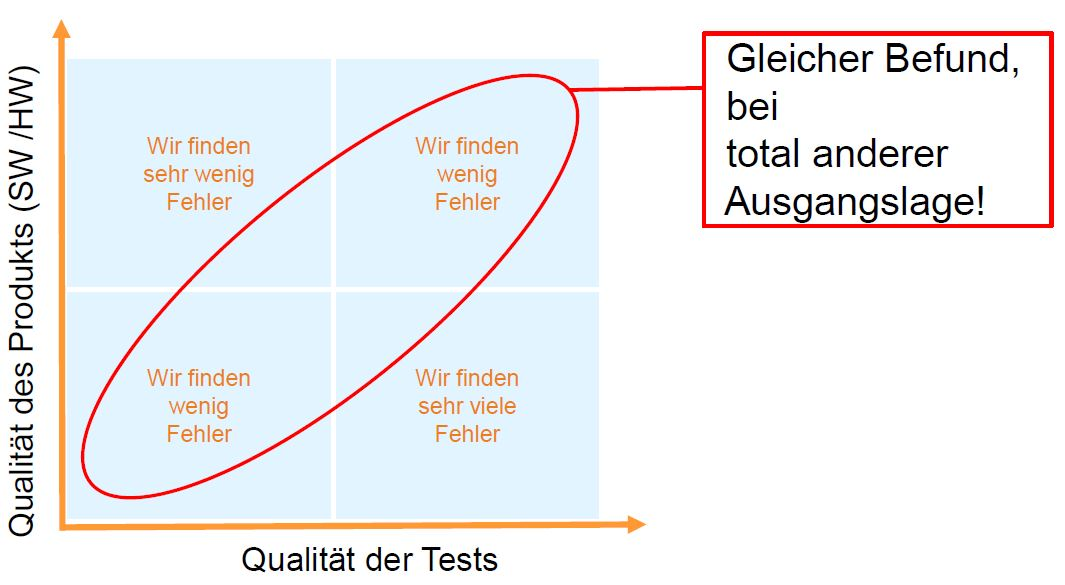
\includegraphics[width=0.7\linewidth]{fig/wichtigkeit-des-testen}
\caption{Wichtigkeit des Testen}
\label{fig:wichtigkeit-des-testen}
\end{figure}

Agile Methoden setzen auf das Testen als Mittel zur Fortschrittsmessung. Schlussendlich wird das Testen innerhalb der Definition of Done formuliert. Ein erfolgreicher Test belegt faktenbasiert, dokumentiert, reproduzierbar und emotionslos, den tatsächlichen Stand/Fortschritt des Projekts. Wobei man im agilen Umfeld mit folgenden Problemen kämpft: Anforderungen nicht sauber definiert, nebst dem Schreiben des Codes geht das Test schreiben unter. Es fehlt die Rolle des Testmanager, kein Reporting. 

\begin{figure}[h!]
\centering
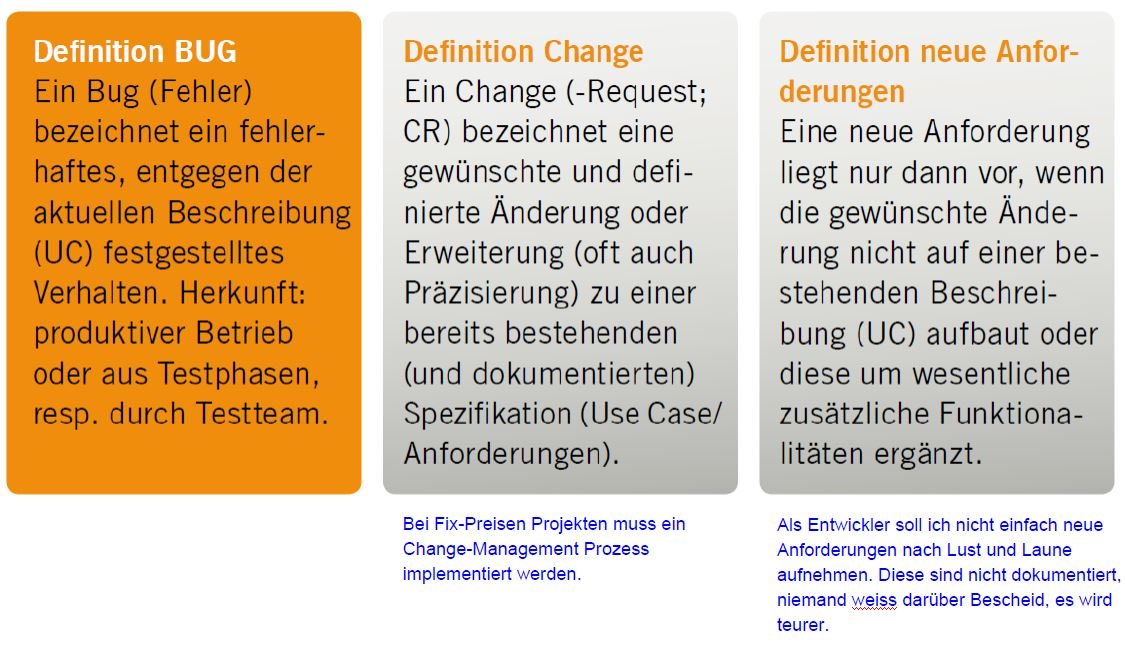
\includegraphics[width=0.7\linewidth]{fig/der-bug}
\caption{Der BUG (MEP!)}
\label{fig:der-bug}
\end{figure}

Ist jeder Fehler ein Fehler? Es macht Sinn die Fehler mit einer Severity (Schweregrad) kategorisieren:
\begin{itemize}
	\item 1 LOW: leichter Fehler, nur einzelne Testschritte betroffen.
	\item 2 MEDIUM: Betriebsstörender Fehler, Systemfunktion nicht beeinträchtig. Wesentlichtes funktioniert.
	\item 3 HIGH: Schwerer Fehler, Auswirkung auf Funktion.
	\item 4 URGENT: Fataler Fehler, Auswirkung auf ganzes System, Testabbruch.
\end{itemize}

Zudem stellt sich immer die Frage ob die Fehler reproduzierbar sind. Man spricht von \textbf{Beobachtungsgüte}:
\begin{itemize}
	\item A: Eindeutig festgestellter, belegbarer und reproduzierbarer Fehler.
	\item B: Nicht ohne weiteres reproduzierbar, aber wiederholt aufgetreten.
	\item C: Nicht reproduzierbar.	
\end{itemize}
